\documentclass{jarticle}
\usepackage[margin={1.5cm, 1.5cm}]{geometry}

\usepackage{listings}
\usepackage{amsmath}
\usepackage{amssymb}
\usepackage{mathtools}
\usepackage{listings}
\usepackage{color}
\usepackage{tabularx}
\usepackage{pdfrender}
\usepackage{bussproofs}
\usepackage[dvipdfmx]{graphicx}
\usepackage{multicol}
\usepackage{hyperref}
\usepackage{breakurl}
\pagestyle{empty}
\usepackage{algorithmic}
\usepackage{algorithm}


\setlength{\columnsep}{1cm}

\title{TFの高性能化とデータ一貫性の確保}
\author{荻原湧志, 川島英之, 大矢晃久, 萬礼応}

\date{}

% 質問をここに書く
% abstractでは\citeは使わない?
% 起承転結が二つ?
% 原文から引用しても良いのか?
% ~の問題がある、は喧嘩腰だろうか?

\begin{document}
% https://puarts.com/?pid=1014
\makeatletter
\newenvironment{tablehere}{\def\@captype{tabel}}{} 
\newenvironment{figurehere}{\def\@captype{figure}}{} 
\makeatother

\maketitle 

\begin{abstract} % 原文から引用
Robot Operating System(ROS)はロボットソフトウェア用のミドルウェアソフトプラットフォームであり、近年多くの研究用ロボットで用いられている。TFライブラリはROSで頻繁に使用されるパッケージであり、ロボットシステム内の座標変換を追跡し、データを変換する標準的な方法を提供するために設計されたものである。ROSの開発初期には複数の座標変換の管理が開発者共通の悩みの種であると認識されていた。このタスクは複雑なために、開発者がデータに不適切な変換を適用した場合にバグが発生しやすい場所となっていた。また、この問題は異なる座標系同士の変換に関する情報が分散していることが多いことが課題となっていた。そこで、TFライブラリは各座標系間の変換を有向森構造として管理し、効率的な座標変換情報の登録、座標変換の計算を可能にした。しかしながら、この有向森構造にはデータの暗黙的な線形補間による一貫性の欠落、及び非効率な並行性制御によりアクセスするスレッドが増えるに従ってパフォーマンスが低下するという問題があることがわかった。そこで、我々はデータベースのトランザクション技術における再粒度ロッキング法、及び並行性制御のアルゴリズムの一種である2PLを応用することにより、この問題を解決した。提案手法では、スレッド数が12までスケールアップすることを示した。また、多くのアクセスパターンにおいて提案手法は既存手法より高いスループットを出すことを示した。
\newline	
\end{abstract}

\begin{multicols}{2}

\section{序論}
\subsection{背景}
% ここもTFの冒頭からコピー
ロボットを使って作業を行う場合、ロボット自身がどこにいるのか、ロボットにはどこにどんなセンサーがついており、また周りの環境のどこにどんなものがあるかをシステムが把握することが重要である。例えば、図\ref{fig:room} のように部屋の中にロボットと、ロボットから観測できる二つの物体があるケースを考える。図中にてロボットは円形、物体は星形で表現される。途中で交わる二つの矢印は各座標系の位置と原点、姿勢を表す。ここでは、地図座標系、ロボットの座標系、二つの物体それぞれの座標系が示されている。
システムはロボットに搭載されたセンサーからのデータを元に各座標系間の位置関係を随時更新する。例えば、自己位置推定プログラムはLiDARから点群データが送られてくるたびにそれを地図データと比較して自己位置を計算し、地図座標系からロボット座標系への位置関係を更新する。物体認識プログラムはカメラからの画像データが送られてくるたびに画像中の物体の位置を計算し、ロボット座標系から物体座標系への位置関係を更新する。
このように、各座標系間の位置関係の更新にはそれぞれ異なるセンサー、プログラムが使われる。各センサーの計測周期、及び各プログラムの制御周期は異なるため、各座標系間の位置関係の更新頻度も異なるものとなる。図\ref{fig:sensor-sync}では、地図座標系からロボット座標系への位置関係データと、ロボット座標系から物体座標系への位置関係データがそれぞれ異なるタイミングで登録されていることを示している。

% SSMはsensor -> osの話で、ROSではosにもう入っていることが前提なのでちょっと話が違うか?

\begin{figurehere} 
\centering
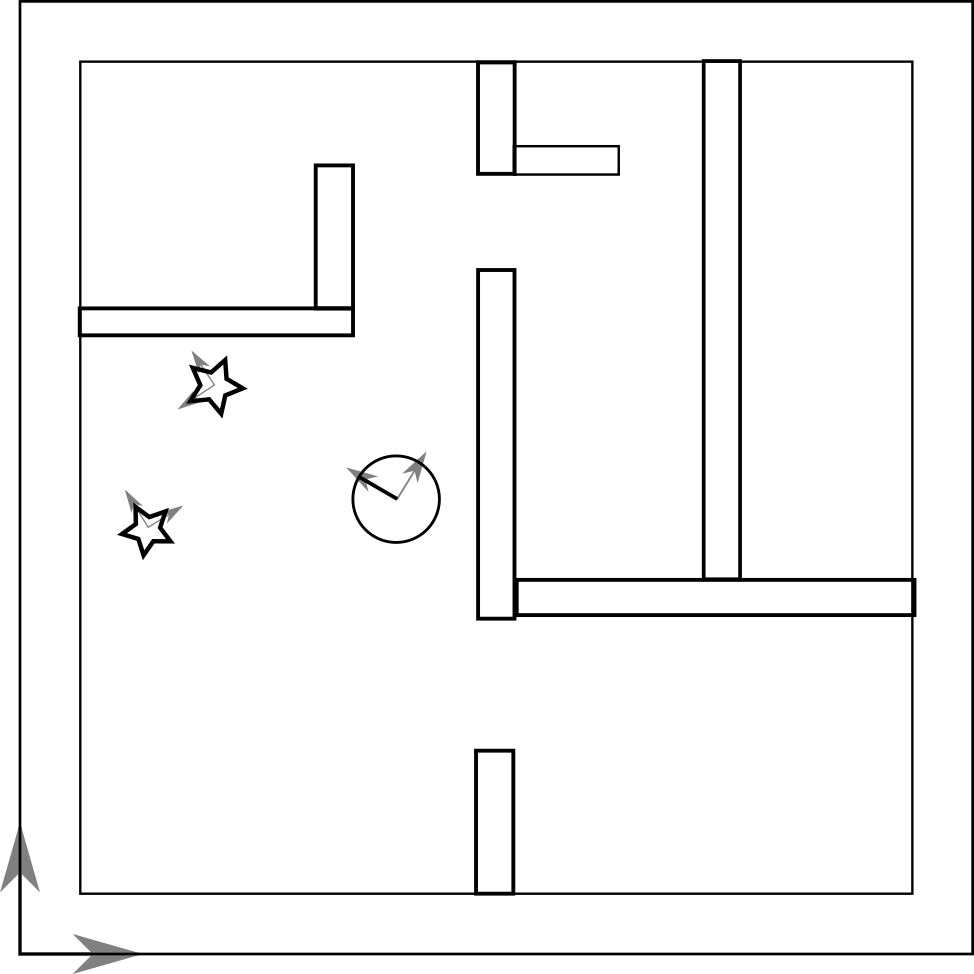
\includegraphics[width=0.3\textwidth]{room}	
\caption{部屋の中のロボット}
\label{fig:room}
\end{figurehere}


\begin{figure*} 
\centering
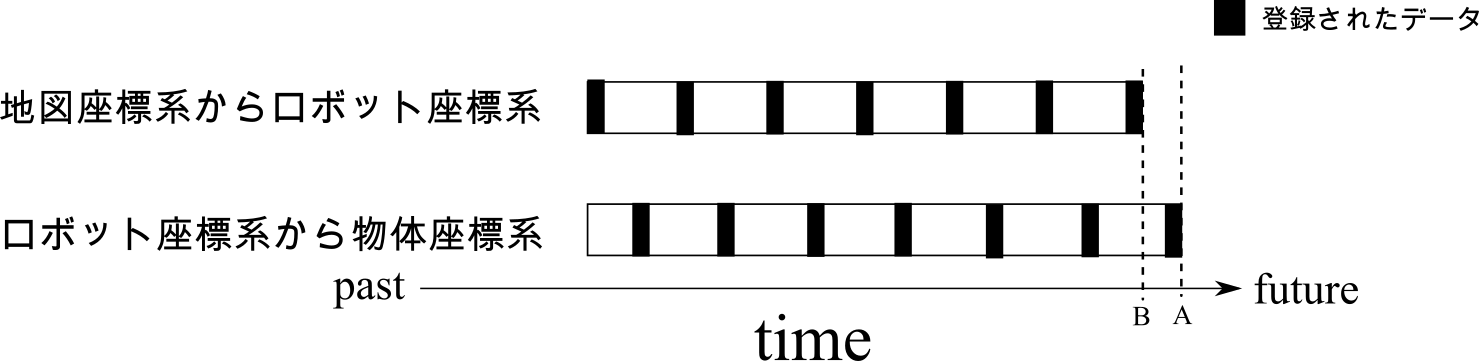
\includegraphics[width=0.8\textwidth]{sensor-sync}	
\caption{位置関係の登録のタイムライン}
\label{fig:sensor-sync}
\end{figure*}


ここで地図中での物体の位置を把握するために、地図座標系から物体座標系への位置関係を取得する方法について考える。地図座標系から物体座標系への位置関係は地図座標系からロボット座標系への変換とロボット座標系から物体座標系への変換を掛け合わせれば計算ができるが、図\ref{fig:sensor-sync}のように各変換

A, Bの選択肢が発生する。AではBのデータが取れないので最後に使われた値を選択するという方法が挙げられる。
BではAのデータが取れないので、



センサの周期、及び

一元管理する必要がある。
またシステム全体について知る必要がある。


Robot Operating System(ROS)\cite{ros}はロボットソフトウェア用のミドルウェアソフトプラットフォームであり、近年多くの研究用ロボットで用いられている。ROSは

この

アームの例を挙げるべきか?

ROSにおいて、次のような問題を解決する必要がある(図を用いながら)




このような同期をどう行うか?
このように、ROSの開発初期には

ここで、TFは森構造で解決をした。
setTransformはいい、lookupTransformだけ
森構造、 10秒のキャッシュ、時系列データ化、

TFライブラリはROSで頻繁に使用されるパッケージであり、ロボットシステム内の座標変換を追跡し、データを変換する標準的な方法を提供するために設計されたものである。Robot Operating System (ROS)の開発初期には複数の座標変換の管理が開発者共通の悩みの種であると認識されていた。このタスクは複雑なために、開発者がデータに不適切な変換を適用した場合にバグが発生しやすい場所となっていた。また、この問題は異なる座標系同士の変換に関する情報が分散していることが多いことが課題となっていた。そこで、TFライブラリは各座標系間の変換を有向森構造として管理し、効率的な座標変換情報の登録、座標変換の計算を可能にした。し


グローバル座標系の中でのロボットの位置、ロボットのローカル座標系の中でのセンサーの位置、センサーのローカル座標系の中での物体の位置、という風に別々に管理している

この時、
グローバル座標系での物体の位置を計算するにはグローバル座標系からロボットの位置の計算 * センサーの位置 * 物体の位置を計算すれば計算できる

TFではこのような座標系同士の変換を次の図のように有向森構造で管理できる。座標系の原点をframeと呼び、このフレームをnode、座標系同士の位置関係を並行移動成分・回転成分でedgeで表した木構造で管理する
木構造で管理することにより、先程のようなグローバル座標系での物体Aの位置は、二つのframe間のパスを辿ることで計算できる
ロボットの座標変換の情報は全てこのTFモジュールで管理される

TFモジュールはROSの多くのパッケージで使われているが、これには以下のような問題点がある

Giant lockにより、木構造が大きくなり多くのスレッドがアクセスするケースでは遅くなる

(setTransformのnon atomicityは実はまだ問題にはならない)

提供されているインターフェイスでは「最新」のデータを取るというメソッドでも実際には該当するパスのデータが完全に準備された状態の時間のデータを返している。

また暗黙的に線形補完が行われるため、データの一貫性がなくなる可能性がある





\subsection{貢献}
そこで、データベースのトランザクション機構における並行性制御のプロトコルの一種である2PLを導入した。

その結果、224コアのマシンではこの程度の性能差が出た

また、データ一貫性を保証できるようなsetTransforms, lookupLatestTransformというインターフェースを導入した。

\subsection{論文構成}
本論文の構成は次の通りである。2章では既存のTF森の構造とその問題点について述べる。3章では提案手法であるTF森の再粒度ロックの導入とデータ一貫性のためのインターフェイスの提供について述べる。4章では提案手法の評価結果を述べる。5章では本研究の結論を述べる。6章では今後の課題について述べる。



\section{関連研究}

TFのようにデータを時系列的に管理するものとしてSSMが挙げられる。

データベースの技術をロボットに適用するという内容ではGAIA\cite{gaia}が挙げられる。

これはRDBベースでreactiveな挙動を提供する。

プロダクトレベルのものを目指すROS2\cite{ros2}やAutoware\cite{autoware}でも、本研究のようなアプローチは存在しない。

2PL以外の並行性制御アルゴリズムとしてはSilo\cite{silo}が挙げられる。



\section{既存のTF森の構造とその問題点}

TF森の実態はtf2パッケージ中にあるBufferCoreクラス\cite{buffer-core} である。
\subsection{構造}
まずはTF森とタイムテーブルから?

各座標系同士の回転移動、並行移動で表現できる位置関係はTF森で表現される

例えば図のようなマップ座標系、ロボット座標系、カメラ座標系、物体の座標系は図のような木構造に対応する。

また、図のフレームA, Bのように他の木とは分離された木が存在してもよい。このため、TF森構造となる。


さて、座標変換の情報は変わらない場合と時刻とともに変わる場合がある

さて、座標変換の情報は主にセンサーからデータが送られてくるたびに計算され、TF森に登録される。このため各フレーム間の座標変換の情報はセンサーの更新頻度に依存し、それぞれ異なるタイミングで更新される。
例えば、マップ座標系からロボット座標系の座標変換を計算するプログラムはLiDARのデータ更新頻度に合わせて自己位置を計算し、マップ座標系からロボット座標系の座標変換を登録する。
カメラ座標系から物体の座標系の座標変換を計算するプログラムはビデオカメラのデータ更新頻度に合わせて物体の位置を計算し、カメラ座標系から物体の座標系の座標変換を登録する。
カメラの更新頻度とLiDARの更新頻度が異なる場合、マップ座標系からロボット座標系の座標変換が登録されるタイミング、カメラ座標系から物体の座標系の座標変換が登録されるタイミングにズレが生じる。マップ座標系から物体の座標系を計算する際にデータ同期の問題が生じてしまう。
これに対処するため、まずTF森は各フレーム間の座標変換情報を過去一定期間保存する。これは図のように表現できる

% map -> robot    
% robot -> camera
% camera -> apple

図は各フレーム間の座標変換情報が提供される時刻を表す。横軸が時間軸を表し、左側が過去、右側が最新の時刻を表す。

灰色線は対応する時刻の座標変換情報が登録されたことを表す。
図の点線の位置でのmapからappleへの座標変換を計算する際、各フレーム間の座標変換情報が必要になる。robotからcameraへの座標変換情報は常にある物として扱われるが、mapからrobot、cameraからappleの座標変換データは該当する時刻では登録されていない。そのため、TFは前後のデータから線形補間を行うことにより座標変換データを計算する。つまり、TFは該当する時刻の座標変換データが保存されている、もしくは前後の値を元に線形補間ができる場合にはその時刻の座標変換データを提供できる、とみなす。





まずはCompactFrameID等のtypedefは説明が面倒なので、展開してしまうか。


座標変換はTransformStorageで表現され、これは以下で構成される
回転成分を表すrotation\_。これはQuaternionで表現される
並行移動成分を表すtranslation\_。これはVector3で表現される
座標変換の時刻を表すstamp。これはros::Time型で表現される
座標変換の親フレームのframe idを表すframe\_id。これは整数型で表現される
座標変換の子フレームのframe idを表すchild\_frame\_id。これは整数型で表現される

TimeCacheInterfaceは特定のフレームから親フレームへの座標変換を登録・管理する抽象クラスである。主に以下のようなメソッドがある
bool getData(ros::Time time, TransformStorage \& data\_out, std::string * error\_str = 0)

特定の時刻timeにおけるTransformStorageを取得する。取得できた場合にはtrueを返し、取得できなかった場合にはfalseを返しエラーの内容をerror\_strに代入する。

bool insertData(const TransformStorage\& new\_data)

座標変換の情報を登録する。情報の登録に成功した場合にはtrueを、そうでない場合にはfalseを返す。

std::pair<ros::Time, CompactFrameID> getLatestTimeAndPare()

最新の座標変換情報のうちその時刻と、親フレームのidを返す。


TimeCacheはTimeCacheInterfaceを継承し、あるフレームにおける親フレームへの座標変換を時系列的に管理する。これはTransformStorageの双方向キューで構成され、ユーザーが座標変換情報を登録する際には先頭にpushし、保存していた座標変換の時刻が10秒以上過去のものとなればdequeから追い出す。getDataのアルゴリズムは以下のようになる


%if(指定した時刻の座標変換データがある){
%  return その座標変換データを返す
%}else{
%  if(前後にデータがある){
%    if(前後で親が同じ){
%       前後のrotationを球面線形補間、前後のtranslationを線形補間したものを返す       
%    }else{
%     エラー
%    }     
%  }else{
%    エラー
%  }
%}




StaticCacheはTimeCacheInterfaceを継承し、先程の例のrobot->sensor間の座標変換のように不変な座標変換情報を管理する。


BufferCoreはTF森を管理する。

文字列であるframeはTF森内部では整数型のidで管理している

TimeCacheInterfaceを継承するTimeCacheとStaticCacheはそれぞれあるフレームからみた親フレームのid、親フレームのの座標変換を保持するため、これらはTF森における子フレームから親フレームへのエッジ及び子フレームのノードを表す。この’ためTF森は子フレームから親フレームへエッジが伸びる有効森構造となっている。


以下のようなインターフェイスがある。
bool setTransform(const geometry\_msgs::TransformStamped\& transform, const std::string \& authority, bool is\_static = false)

座標変換情報を登録する。authorityには座標変換情報を登録するプログラムの名前等を指定できる。is\_staticをtrueにすると、StaticCacheにデータを登録できる。
下記の更新、挿入において詳細を説明する

geometry\_msgs::TransformStamped lookupTransform(const std::string\& target\_frame, const std::string\& source\_frame, const ros::Time\& time) const;
		   
時刻timeにおけるtarget\_frameからsource\_frameへの座標変換を返す。
下記の検索の節において詳細を説明する


template<typename F> int walkToTopParent(F\& f, ros::Time time, CompactFrameID target\_id, CompactFrameID source\_id, std::string* error\_string) const;


指定の時刻timeについてtarget\_idからsource\_idへの座標変換を計算する。返り値は0以外の場合にはエラーコードとなり、エラーの原因がerror\_stringに代入される。

テンプレートパラメータのFにはよくTransformAccumクラスが与えられ、これは通過したパスの座標変換情報を蓄積するオブジェクトである。

主にlookupTransformの中で用いられる。

int getLatestCommonTime(CompactFrameID target\_frame, CompactFrameID source\_frame, ros::Time\& time, std::string* error\_string) const;

target\_frameからsource\_frameまでのパスにおいて、座標変換のデータが提供できる時刻で最新のものを取得する。そのような時刻が存在する場合にはtimeに代入され0を返す。もしそのような時刻がない場合にはエラーコードを返し、エラーの内容をerror\_stringに代入する。

これは図のように説明できる。

図においてmapからrobotへのパスにおいて必要なのはmapからrobotへの座標変換、robotからsensorへの座標変換。sensorからappleへの座標変換である。この中で最新のデータが最も古い時刻に来ているのはmapからrobotへの座標変換である。この時刻よりも前ならばmapからappleへの座標変換データは提供できるが、この時刻より後ではパス中の座標変換が提供できなくなる。このため、getLatestCommonTimeではこの時刻Aが選択される。

ここで、図中ではlidarからobjectへの座標変換が最も古い時刻に来ているが、mapからrobotへの座標変換を計算する時にこの座標変換は使わないために時刻Dが選ばれないことに注意する。

(robot -> lidar -> とか別のもっと遅いものも追加!)

TimeCacheInterfacePtr BufferCore::getFrame(CompactFrameID frame\_id)

与えられたframe\_idに対応するTimeCahceInterfaceへのポインタを取得する。該当するものがない場合にはnullを返す。

また、BufferCoreには以下のようなフィールドがある



frames\_: 各フレームidに対応するTimeCacheInterfaceのポインタを管理する配列。TF森はこの配列で表現される。




frameからframe idを検索するテーブル、及びframe idからframeを検索するテーブルが存在する frameIDs\_, frameIDs\_reverse

frame\_mutex\_: frames\_, frameIDs\_, frameIDs\_reverseは複数のスレッドから操作される。データ競合を防ぐため、各スレッドはframe\_mutex\_を用いて排他処理を行う。


特定のフレームに対応するTimeCacheInterfaceを取得するには、まずframeIDs\_から対応するframe idを取得し、続いてframes\_から対応するTimeCacheInterfaceへのポインタを取得する。この二回の検索処理の後、TF森のフレームに該当するTimeCacheInterfaceにアクセスできる。

TransformAccumクラスは、lookupTransformにて木構造を辿って座標変換を計算する際に座標変換の計算を蓄積していくクラスである。

int gather(TimeCacheInterface* cache, Time time, string * error\_string)

cacheからtimeの時の座標変換を取得し、それをTransformAccumインスタンス内の一時変数に記録する。cacheから親のフレームのidを取得しそれを返す。	


\subsection{lookupTransform}

擬似コード

\begin{algorithm}[H]
	\caption{lookupTransform}
	\begin{algorithmic}
	\STATE e = walkToTopParent
	\IF{$n < 0$}
	\STATE $X \leftarrow 1 / x$
    \STATE $N \leftarrow -n$
    \ENDIF
	\end{algorithmic}
\end{algorithm}


まずはrunning exampleを示す。なるべくC++レベルでの説明は避けるべきか。
とりあえず、途中で親が変わらないと仮定する。じゃないと説明が面倒

1. sourceからrootへの座標変換を計算
2. targetからrootへの座標変換を計算
3. sourceからrootへの座標変換 * rootからtargetへの座標変換を計算

まずは普通のケースから。同じ親を持ち、
%    r
%   / \
%  /   \
%  a     c
% / \
% b e
%/
%d
%
% d -> e
まずはこの時間で見ていく
まずはdからrへの座標変換を計算
次にeからrへの座標変換を計算
rからeへの座標変換は、単にeからrへの逆変換をとれば良い。
あとはdからrへの変換 * rからeへの変換で計算できる

% r
% |
% t
% |
% s

このようにtargetが直接の

ここら辺は説明省いても良い????

この例のように、sourceとtargetが同じ木の中にない場合、つまり同じrootを共有しない場合にはエラーとなる。


running exampleが十分であれば、擬似アルゴリズムでの説明を省けるかも。

\begin{algorithm}[H]
	\caption{walkToTopParent(time, source\_id, target\_id)}
	\begin{algorithmic}
	\STATE frame\_id = source\_id
	\STATE top\_parent\_id = frame\_id
	\STATE // source frameからrootへのパスをたどる
	\WHILE{ frame\_id $\neq$ 0 }
	\STATE cache = getFrame(frame\_id)
	\IF{cache = NULL}
	\STATE // 木構造のrootに到達
	\STATE top\_parent\_id = frame\_id
	\STATE \textbf{break}
	\ENDIF
	\STATE paret\_id = cacheから座標変換と親のidを取得
	\IF{frame\_id == target\_id }
	\STATE // target frameはsource frameの祖先なので早期リターン
	\STATE 累積したデータから座標変換を計算
	\RETURN 0
	\ENDIF
	\STATE 座標変換を蓄積
	\STATE top\_parent\_id = frame\_id
	\STATE frame\_id = parent\_id
	\ENDWHILE
	
	\STATE // target\_idからrootへのパスをたどる
	\STATE frame\_id = target\_id
	\WHILE{ frame\_id $\neq$ top\_parent\_id }
	\STATE cache = getFrame(frame\_id)
	\IF{cache = NULL}
	\STATE // 木構造のrootに到達
	\STATE \textbf{break}
	\ENDIF
	\STATE parent\_id = cacheから座標変換と親のidを取得
	\IF{frame\_id == source\_id }
	\STATE // source frameはtarget frameの祖先なので早期リターン
	\STATE 累積したデータから座標変換を計算
	\RETURN 0
	\ENDIF
	\STATE 座標変換を蓄積
	\STATE frame\_id = parent\_id
	\ENDWHILE
	\IF{frame\_id $\neq$ top\_parent\_id}
	\STATE // source frameとtarget frameは同じ木構造に属していない
	\RETURN エラーコード
	\ENDIF
	\STATE // source frameとtarget frameは祖先関係にはないが、同じ木に属している
	\STATE source frameからtarget frameへの座標変換の計算
	\RETURN 0
	\end{algorithmic}
\end{algorithm}




\subsection{setTransform}

座標変換を登録する。特に説明の必要はない

\subsection{問題点}

ここより上の部分では、どの程度エラーケースを、どの程度正確な説明が必要か不明瞭。とりあえず以下を書き下す。

giant lock

最新のデータを返さない
exampleを示そう
%
% a  |  | |
% b    | 
% c   | | 
この場合には、bに引っ張られてaの最新のデータが取れない

線形補間により、一貫性がないケースがある。
例えば関節間の制約やジンバルロック、特異点など
制御プログラムが意図しない状態を見てしまうかもしれない

\section{提案手法}

まず、ginat lockをしない方法を導入
読み書きを行う際には必要なノードのみlockする

setTransformとは異なり、lookupTransformは各ノードの情報の読み込みのみ行う。

読み込み処理であれば複数のスレッドからの同時アクセスを行ってもdata raceは発生しない。このため、


S lockはdata raceが発生しないreadの時に、X lockは二つ以上のスレッドからwrite操作されるとdata raceが発生するのを防ぐために使われる。

(S-Xはもう古い?readとwriteの方が説明が適切?)


さらに、shared lockとexclusive lockを導入する
これは次のような表で表現できる
%   N | S | X
% S o   o   x   
% X o   x   x
%
表は列が既にかかっているロック(Nは何もかかっていない)、行はかけようとしているロックを表し、oであれば新たにかけようとしているロックの確保に成功し、xであればロックがかけられないことを表す
例えば、S lockが既にかけられていても新たにS lockを他のスレッドが書けることが可能になる。対し、X lockが既にかかっている場合にはS lockはかけられず、S lockがかかっている場合にもX lockはかけられない。X lockをかけることができるスレッドは常に一つだけである。


続いて、最新のデータを取らない問題と線形補間によりデータの一貫性がなくなる問題について

既存のlookupTransformでは、最新のデータを取得しようとしても過去のデータを参照してしまう、また線形補間されてしまう

最新のデータをそれぞれ取ってくるという方法もサポートする。(しかしこれだけでは十分ではない。 <- このsつ名の導入はいまいち。)冒頭で説明したように、ROSは分散アーキテクチャを採用する。TFMessageには各フレーム間の座標変換情報を複数登録できるが、TFは複数の座標変換をsetTransformを複数回呼び出すことにより実現している。これにより、中間の状態を見てしまう。これは図のように説明できる。
この図のように、giant lockを毎回のsetTransformで取ってはいるが、その操作が終わり次のsetTransformsを呼ぶまでの間はlockが外される。これにより、一貫性のない状態を見てしまう恐れがある。


そこで、我々は最新のデータをatomicに取得するlookupLatestTransform、及び複数の座標変換を一度にatomicに登録できるseTransformsを追加した。複数のデータに対する読み込み、書き込みをatomicに行うために、我々は2PL[?]を実装した。

しかしながら2PLにはdead lockの問題がある。
例えば次の例、これは木を登る方向と下る方向の両方があるからこうなる。

データをreorderできれば2PLではdeadlockは発生しない(DAGが構築できる)、がTF木ではできそうにない。

そこで我々はdeadlock preventの方法としてNo-wait[Bern 1981]を採用した。これはwrite lockをかけようとして失敗したら最初からやり直す。

Wound wait, nonpreemptive (Concurrency Control in Distributed Database Systems PHLIP.A BERNSTEIN AND NATHAN GOODMAN P196)

transactionにpriorityを足すとかは?



\section{評価}
実験を行う

スレッド数を上げるとスループット伸びる
jointを増やすと緩やかにスループットが落ちる
iterを増やすと1000以降で急激にスループットが下がる。no waitによる弊害か?lockの確保に失敗しているのかも
read ratioは高くなるほどブロックされる可能性が減る
read lenは安定しているように見える。なぜtrnでread lenが小さいとこうなるのか。。。2PLでロックする箇所が変わるから?

write lenを上げるとやはりブロックされる部分が増える



\section{結論}

再粒度ロックの導入により、パフォーマンスを上げることができた
特に、スレッド数の増加とともにスループットが下がる問題を解決できた

データの一貫性は必須、というデータも示したい。

\section{今後の課題}

ここでは取り上げなかったTF木の問題点として、部分的に座標情報の登録に失敗するケース。rollbackなどもいれtransactionalに行う必要

また、insert/deleteが大量に発生するケースも考える。

	
\begin{thebibliography}{99}

\bibitem{ros} M. Quigley, K. Conley, B. P. Gerkey, J. Faust, T. Foote, J. Leibs, R. Wheeler, and A. Y. Ng, “Ros: an open-source robot operating system,” in ICRA Workshop on Open Source Software, 2009.

\bibitem{tf} T. Foote, "tf: The transform library," 2013 IEEE Conference on Technologies for Practical Robot Applications (TePRA), 2013, pp. 1-6, doi: 10.1109/TePRA.2013.6556373.

\bibitem{2PL} Philip A. Bernstein and Nathan Goodman, "Concurrency Control in Distributed Database Systems" in ACM Computing Surveys, 1981, pp. 185-221

\bibitem{buffer-core} "BufferCore.h", \url{https://github.com/ros/geometry2/blob/noetic-devel/tf2/include/tf2/buffer_core.h}

\bibitem{gaia} "GAIA platform", \url{https://www.gaiaplatform.io}

\bibitem{ros2} "ROS2", \url{https://docs.ros.org/en/rolling/}

\bibitem{autoware} "Autoware", \url{https://tier4.jp/en/autoware/}

\bibitem{silo} Stephen Tu, Wenting Zheng, Eddie Kohler †, Barbara Liskov,
and Samuel Madden. Speedy transactions in multicore in-memory
databases. In SOSP, pages 18–32. ACM, 2013

\end{thebibliography}
	
\end{multicols}	
\end{document}
